\section{Introduction}

% Topology is the wildest in d=4. QFT is an important tool to
% tackle it.
Topology is probably the wildest in dimension four. For example,
the cardinality of the set of smooth structures on
$\mathbb{R}^{n}$ (up to equivalence) is $1$ unless $n=4$ in which
case there are uncountably many; Poincare conjecture remains
wildly unproven only for $n = 4$.. etc. Some tools can help
tackle to some extent: Donaldson invariants, Seiberg-Witten
invariants, and Yamabe invariants are shown to be sensitive to
exotic smooth structures for some special cases. Despite their
successes, they were known not to be fully sensitive, and were
hard to modify because they include heavy analytic packages.

In the $90$s, another simpler invariant for smooth $4$-manifolds
was proposed by Crane and Yetter. However, it was soon known to
be too ``weak'' in the sense that it only sees the homotopy type.
However, its simplicity leaves more space for modification.
Though several attempts have been made
\cite{barenz/evaluation-crane-yetter}, not much success has been
achieved yet in terms of sensitivity to exotic smooth structures.
A recent work by Reutter \cite{reutter/semisimple} explains the
failure, suggesting that we need a non-semisimple variant of CY
model for the goal.

Before moving on to a non-semisimple CY model, the author decides
to investigate another model for $4$D topology, the Turaev shadow
model. The shadow model originated from the face model in
statistical mechanics, and it was known to coincide with the CY
model in some cases in which the $4$D CY model degenerates to the
$3$D Witten-Reshetikhin-Turaev model
\cite{barrett/observables-in-tv-and-cy}. It is thus natural to
study the difference between the shadow model and the CY model in
a more general setting \footnote{If based on a modular tensor
  category, the CY model degenerated to the WRT model. By a more
  general setting we mean the CY model with the based on a
  premodular category (i.e. modular except the $S$-matrix could
  be degenerate).}.

This work shows that there is no such difference, suggesting the
community again to move on and pursue an effective non-semisimple
CY model. Along proving the equivalence of the two models, we
make heavy use of the construction of the Turaev shadow model
first given in the big book \cite{turaev-qiok-3-manifolds}, in
which the model is defined over any modular tensor category. We
observe that the model can be extended to the premodular case.

\subsection{Sections summary}

\begin{itemize}
  \item Section \ref{section/algebra}: The basics of tensor
        categories, their graphical calculi and tensor networks,
        and special numerical entities ($n$j-symbols). Nothing in
        this section is new.
  \item Section \ref{section/topology}: Three kinds of data that
        present smooth $4$-manifolds: triangulations, handle
        decompositions, and shadows. We also fully recall the
        definition of a shadow, which closely resembles foams in
        the modern literature. Nothing in this section is new.
        Readers can treat this paper as a thin interface to the
        book.
  \item Section \ref{section/sum}: Definitions of the two state
        sums: the CY model and the shadow model. The observation
        that the shadow model can be extended from modular
        categories to premodular categories is new. We conclude
        the section by stating and proving the equivalence.
\end{itemize}

\subsection{Note on the arXiv version}
The tex source file of this paper includes hidden details, which
can be displayed by recompiling with toggling \texttt{details} in
the source.

\subsection{A summary to experts}\label{subsection/a-summary-to-experts}

The idea of the proof for the equivalence is simple. Let $X$ be a
$4$-manifold. While the CY state sum can be computed from any
triangulation $T$ of $X$, the shadow state sum can be computed
from any stable shadow of $X$. We construct a natural stable
shadow $S$ from $T$ and compute the shadow sum in terms of $S$.
By the locality of shadow sum, we reduce the task to proving that
the local shadow evaluates to the local term involved in the CY
state sum (namely, the $10$j-symbols). This is proven in
\ref{lemma/10j-symbol-as-shadow-state-sum}.

\subsection{Conventions}

\noindent Some conventions we use globally in the paper:

\begin{itemize}
  \item We fix a algebraic closed field $\mathbb{k}$ of
        characteristic $0$.
  \item By a vector space $V$ we mean a finite dimensional vector
        space over the field $\mathbb{k}$, unless further
        specified. The linear dual
        $Hom_{\mathbb{k}}(V,\mathbb{k})$ is denoted by
        $V^{\star}$.
  \item By a manifold we mean a piecewise-linear, oriented,
        connected and closed manifold in real dimension $4$
        unless further specified.
  \item In this paper, by a monoidal category we mean a strict
        monoidal category (we do not lose any generality by Mac
        Lane's strictness theorem). \details{For the statement
        and a full modern proof, see \cite[theorem
        2.8.5]{egno/tensor-cats}.}
\end{itemize}

\section{Algebra $(A)$}\label{section/algebra}
\subsection{Premodular category}

The full definition of a premodular category from scratch is
tedious. Unfamiliar readers can think of a premodular category
roughly as a higher version of the group algebra of a finite
group. A formal definition can be found after some motivations
(\ref{def/premodular-category}).

Algebraic objects help abstract details in various mathematical
problems. However, they sometimes abstract too much to recover
information of interest. In recent years, mathematicians
``categorify'' algebraic objects in order to retain more
information. For example, a ring is categorified to a tensor
category, and a tensor category with special properties and
additional structures could be powerful. For example, a ribbon
fusion category provide quantum invariants of knots that
generalize the Jones polynomials. A premodular category is a
braided fusion category satisfying with a spherical structure.
Examples include the (modified) category of representations of
finite groups, finite $2$-groups, and quantum groups.

\begin{definition}[premodular category]\label{def/premodular-category}
  A premodular category is a spherical braided fusion category.
\end{definition}

\noindent In particular, a premodular category $C$ is semisimple,
$\mathbb{k}$-linear, and fusion. Define its set of simples to be
the set $I$ of simple $C$-objects up to isomorphism. Denote
$0 \in I$ so that the monoidal identity $\mathbb{1} \in 0$. As
taking monoidal dual preserves simplicity, for each $i \in I$
there is a unique element $i^{\star}$ in $I$ such that
$V_{i}^{\star} \in i^{\star}$ whenever $V_{i} \in i$. So $I$ is a
finite set with an involution $I \xrightarrow{\star} I$. Using
the spherical structure, we can define for each $i \in I$ the
number $dim_{C}(i) = dim(i) \in \mathbb{k}$ as the trace of
$id_{V_{i}}$ and the number $\nu_{i} \in \mathbb{k}^{\star}$ as
the twisting coefficient $tr(\theta_{V_{i}})/tr(id_{V_{i}})$,
where $\theta_{V_{i}}$ denotes the endomorphism of $V_{i}$
depicted in the following graph.
\begin{center}
  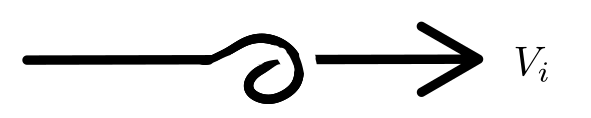
\includegraphics[height=0.8cm]{twist}
\end{center}
We further define the Gauss sum of $C$ to be
$$\Delta_{C} = \sum_{i \in I} \nu_{i}^{-1}dim(i)^{2}.$$

\noindent In order to do computations with a premodular category
we need to choose and fix some extra data (called a coordinate).
All intrinsic results are independent of the choice.

\begin{definition}[coordinated premodular
  category]\label{def/coordinated-premodular-category}
  Let $C$ be a premodular category and $I$ its set of simples.
  Choose and fix the following:
  \begin{itemize}
    \item A number $D \in \mathbb{k}$ such that
          $D^{2} = \sum_{i \in I} dim_{C}(i)^{2}$ (the global
          dimension of $C$).
    \item A set of $C$-objects $\{V_{i}\}_{i \in I}$ such
          that $V_{i} \in i$ and that $V_{0} = \mathbb{1}$.
    \item A set of isomorphisms [(p.313)]
          $\{\omega_{i}: V_{i} \to (V_{i^{\star}})^{\star}\}_{i \in I}$.
    \item A set of numbers
          $\{dim_{C}'(i) = dim'(i) \in \mathbb{k}\}_{i \in I}$
          such that $dim_{C}'(0) = 1$,
          $dim_{C}'(i)^{2} = dim_{C}(i)$, and
          $dim_{C}'(i^{\star}) = dim_{C}'(i)$.
    \item A set of numbers
          $\{\nu_{i}' \in \mathbb{k}\}_{i \in I}$ such that
          $\nu_{0}' = 1$, $(\nu_{i}')^{2} = \nu_{i}$, and
          $\nu_{i^{\star}}' = \nu_{i}'$ [(p.313)].
  \end{itemize}

  Such a $5$-tuple
  $\vec{d} = (D, \{V_{i}\}, \{\omega_{i}\}, \{dim'(i)\}, \{\nu'_{i}\})$
  is called a coordinate of the premodular category $C$. Such a
  pair $(C, \vec{d})$ is called a coordinated premodular
  category.
\end{definition}

\noindent We will often confuse a premodular category with a
coordinated premodular category.

\begin{definition}[multiplicity module]\label{def/multiplicity-module}
  Let $C$ be a (coordinated) premodular category and $I$ its set
  of simples. Respectively, define $H^{ijk}$, $H_{k}^{ij}$, and
  $H_{ij}^{k}$ to be the $\mathbb{k}$-modules
  $Hom_{C}(\mathbb{1}, V_{i} \otimes V_{j} \otimes V_{k})$,
  $Hom_{C}(V_{k}, V_{i} \otimes V_{j})$, and
  $Hom_{C}(V_{i} \otimes V_{j}, V_{k})$.
\end{definition}

\noindent We identify $H_{k}^{ij}$ with $H^{ijk^{\star}}$ and
$H_{ij}^{k}$ with $H^{kj^{\star}i^{\star}}$ by the linear maps
induced by the following graph and call them the canonical
identifications:
\begin{center}
  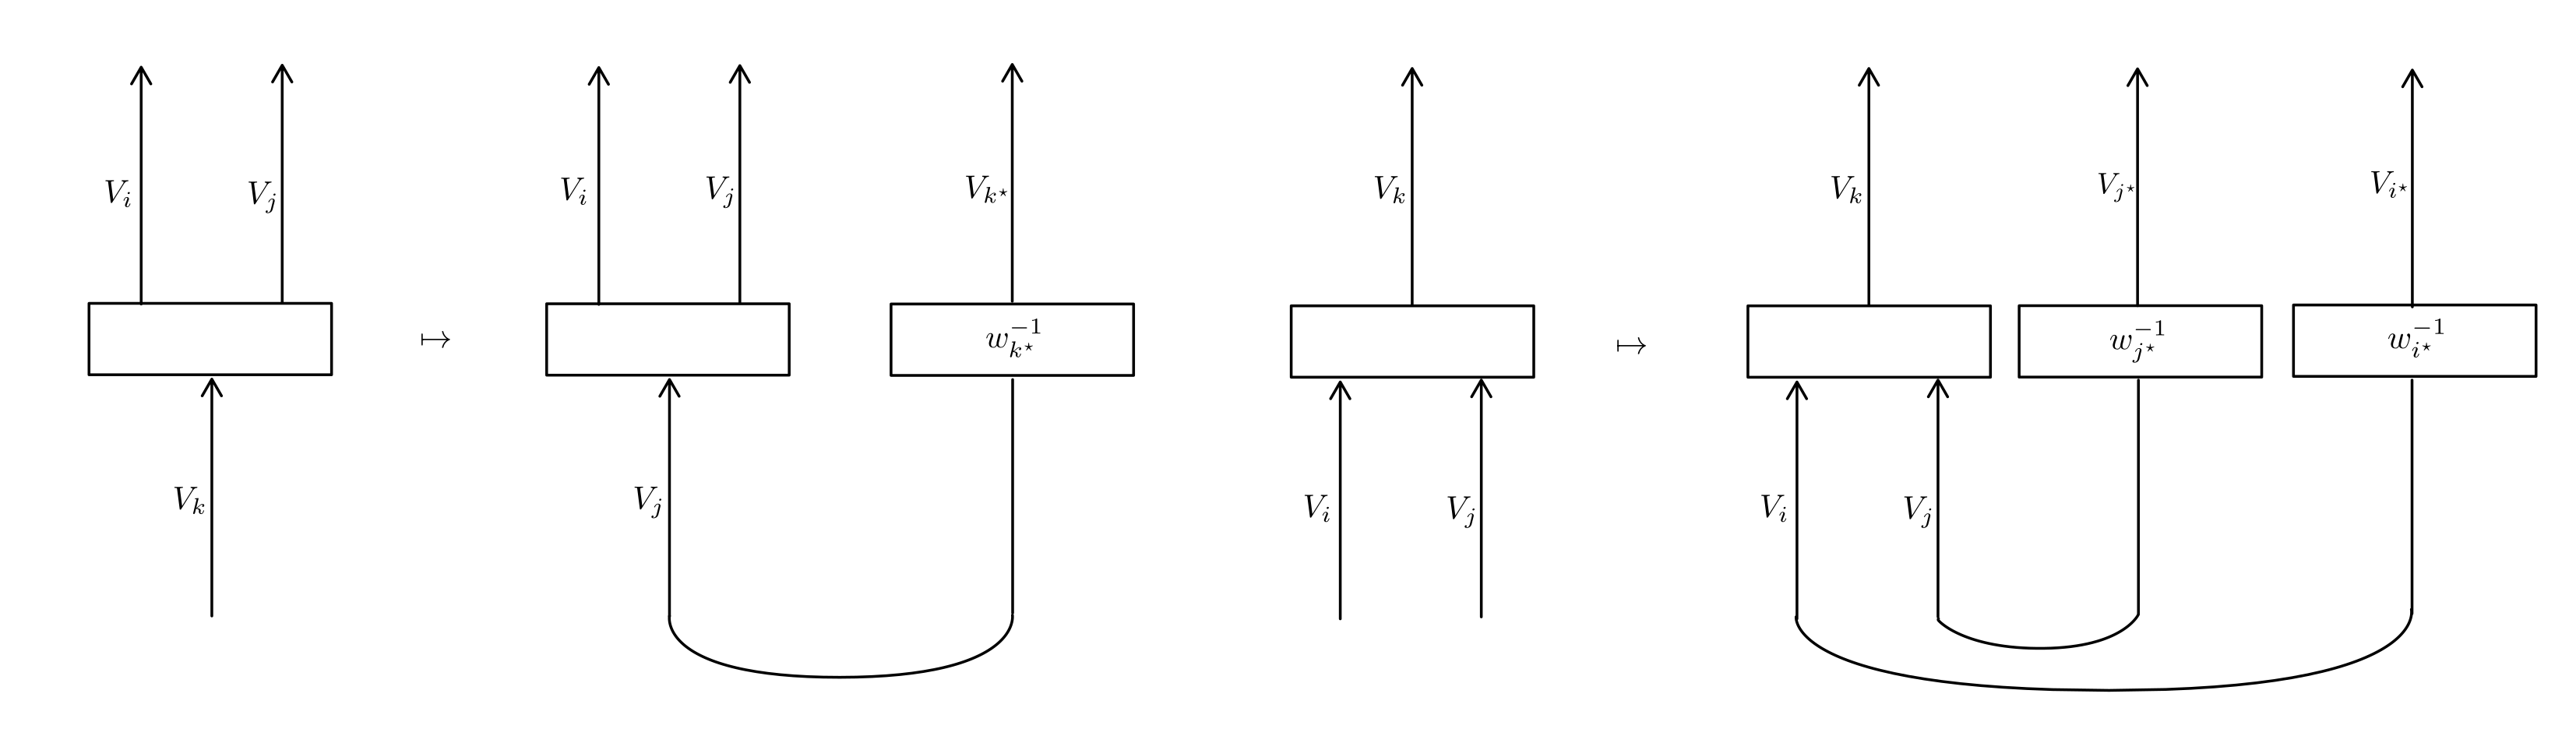
\includegraphics[height=5.5cm]{identification}
\end{center}
\noindent Recall that the natural pairing
$$H^{ij}_{k} \otimes_{\mathbb{k}} H_{ij}^{k} \to Hom_{C}(V_{k},V_{k}) \xrightarrow{tr} \mathbb{k})$$
is nondegenerate by the semisimplicity of $C$. The braided
structure of $C$ guarantees that the $\mathbb{k}$-modules
$H^{ijk}$, $H^{ikj}$, $H^{jik}$, $H^{jki}$, $H^{kij}$, $H^{kji}$
are all isomorphic. In category theory, we must carefully
distinguish equalities from isomorphicities, hence we introduce a
way to keep track of the isomorphisms among the $H^{ijk}$'s.

\begin{definition}[canonical isomorphisms]\label{def/canonical-isomorphism}
  Let $C$ be a premodular category, $c$ its braided structure,
  $I$ its set of simples, and $i,j,k \in I$. Define the
  canonical isomorphisms
  $H^{ijk} \xrightarrow{\sigma_{1}(ijk)} H^{jik}$ and
  $H^{ijk} \xrightarrow{\sigma_{2}(ijk)} H^{ikj}$ by
  $$\sigma_{1}(ijk): \phi \mapsto \nu_{i}'\nu_{j}'(\nu_{k}')^{-1}(c_{V_{i}, V_{j}} \otimes id_{V_{k}})\phi,$$
  $$\sigma_{2}(ijk): \phi \mapsto \nu_{j}'\nu_{k}'(\nu_{i}')^{-1}(id_{V_{i}} \otimes c_{V_{j}, V_{k}})\phi.$$
\end{definition}

\noindent It is a simple exercise in the theory of tensor
categories to check that
\begin{equation} \label{eq1}
  \begin{split}
    \sigma_{1}(jik)\sigma_{1}(ijk) & = id, \\
    \sigma_{2}(ikj)\sigma_{2}(ijk) & = id, \\
    \sigma_{1}(jki)\sigma_{2}(jik)\sigma_{1}(ijk) & = \sigma_{2}(kij)\sigma_{1}(ikj)\sigma_{2}(ijk)
  \end{split}
\end{equation}
so $\sigma_{1}$ and $\sigma_{2}$ specify the isomorphisms among
the six $\mathbb{k}$-modules.

\begin{definition}[symmetrized multiplicity module]\label{def/symmetrized-multiplicity-module}
  Let $C$ be a premodular category, $I$ its set of simples, and
  $i, j, k \in I$. Define the symmetrized multiplicity module
  $H(i,j,k)$ to be the $\mathbb{k}$-module consisting of
  functions $\phi$ that assign an element
  $\phi^{i_{1}i_{2}i_{3}} \in H^{i_{1}i_{2}i_{3}}$ to each
  ordering $(i_{1}, i_{2}, i_{3})$ of the set $\{i, j, k\}$.
\end{definition}

\noindent The point is that all the symmetrized modules
$H(i,j,k)$, $H(i,k,j)$, $H(j,i,k)$, $H(j,k,i)$, $H(k,i,j)$,
$H(k,j,i)$ are \textit{equal as sets}. By definition, there is a
canonical identification between $H(i,j,k)$ and $H^{ijk}$.

\begin{definition}[contraction]\label{def/contraction}
  Let $C$ be a (coordinated) premodular category, $I$ its set of
  simples, and $i, j, k \in I$. Define the contraction map
  $H^{ijk} \otimes H^{k^{\star}j^{\star}i^{\star}} \to \mathbb{k}$
  by the following diagram \details{\cite[figure
    VI.3.5]{turaev-qiok-3-manifolds}}
  \begin{center}
    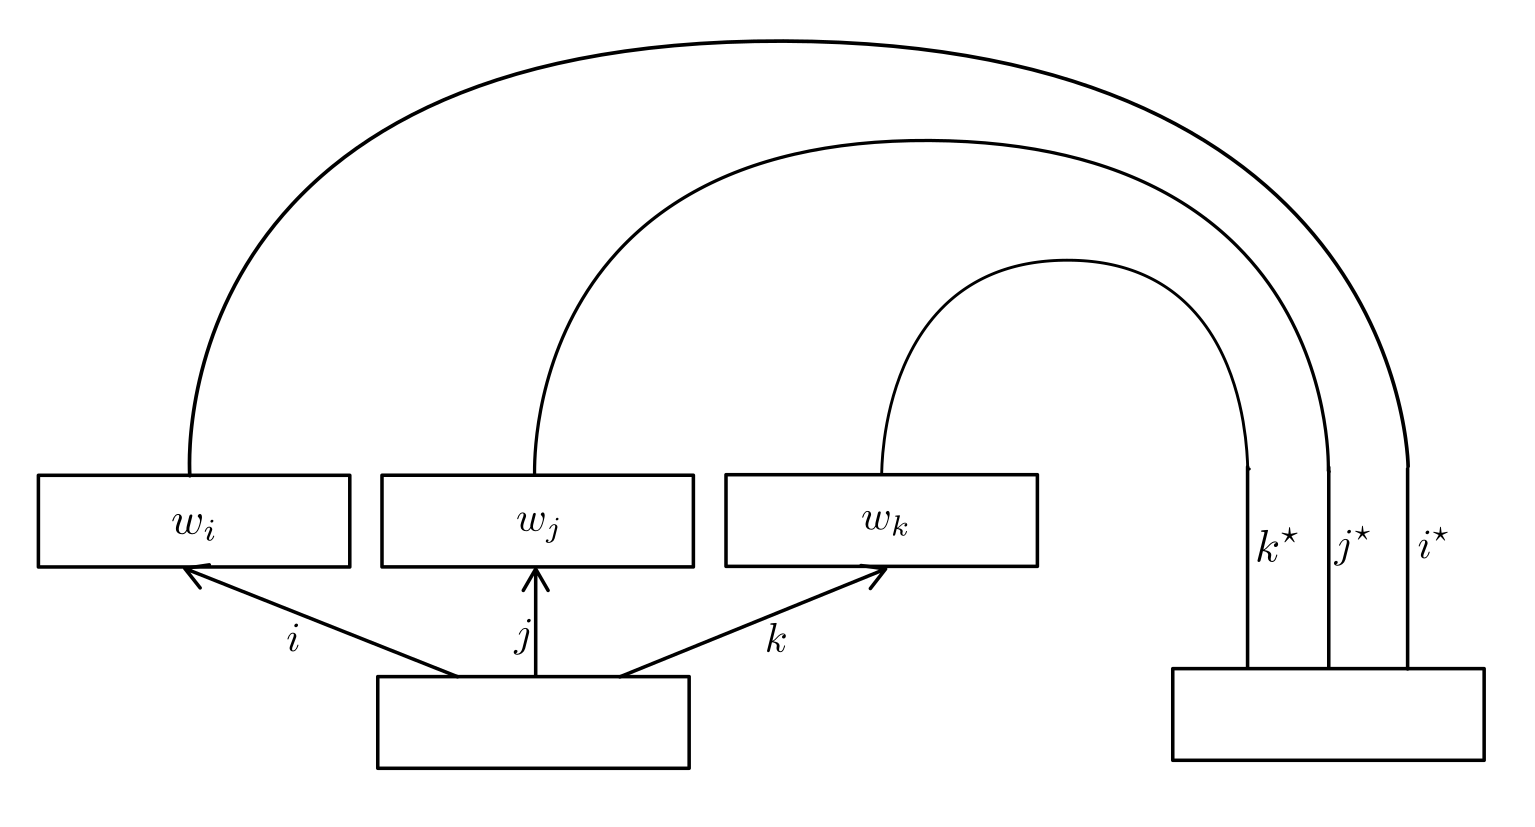
\includegraphics[height=6cm]{pairing}
  \end{center}
  Denote the canonically induced contraction map on the
  symmetrized modules to be (p.334)
  $$\ast_{ijk}: H(i,j,k) \otimes_{\mathbb{k}} H(i^{\star}, j^{\star}, k^{\star}) \to \mathbb{k}.$$
  This defines a nondegenerate pairing and thus induces a
  canonical element $Id(i,j,k)$ in the domain of $\ast_{ijk}$
  (p.333).
\end{definition}

\noindent We will abuse notation by denoting natural contractions
from the non-ordered tensor products
$V \otimes_{\mathbb{k}} H(i,j,k) \otimes_{\mathbb{k}} H(i^{\star}, j^{\star}, k^{\star})$
to $\mathbb{k}$ by $\ast_{ijk}$ for any $\mathbb{k}$-module $V$.

\subsection{$6$j-symbol, $10$j-symbol, and $15$j-symbol}

\newcommand{\sixJSymbol}[6]{\begin{bmatrix}
  #1 & #2 & #3 \\
  #4 & #5 & #6 \\
\end{bmatrix}}

\newcommand{\normalizedSixJSymbol}[6]{\begin{vmatrix}
  #1 & #2 & #3 \\
  #4 & #5 & #6 \\
\end{vmatrix}}

% Used as in \tenJSymbol{a}{b}{c}{d}{e}{f}{g}{{h}{i}{j}}
\newcommand{\tenJSymbol}[8]{\begin{vmatrix}
    #1 & #2 & #3 & #4 \\
     * & #5 & #6 & #7 \\
    \tenJSymbolContinued #8 \\
  \end{vmatrix}_{10j}
}

\newcommand\tenJSymbolContinued[3]{
  * & * & #1 & #2 \\
  * & * & * & #3
}

\begin{definition}[$6$j-symbol]\label{def/6j-symbol}
  For each $i,j,k,l,m,n \in I$, we define the $6$j-symbol
  $$\sixJSymbol{i}{j}{k}{l}{m}{n}:
  H_{k}^{ij} \otimes H_{m}^{kl} \otimes H_{jl}^{n} \otimes H_{in}^{m} \to \mathbb{k}$$
  to be the linear map induced by the partial tensor network on
  the $2$-sphere $S^{2}$:
  \begin{center}
    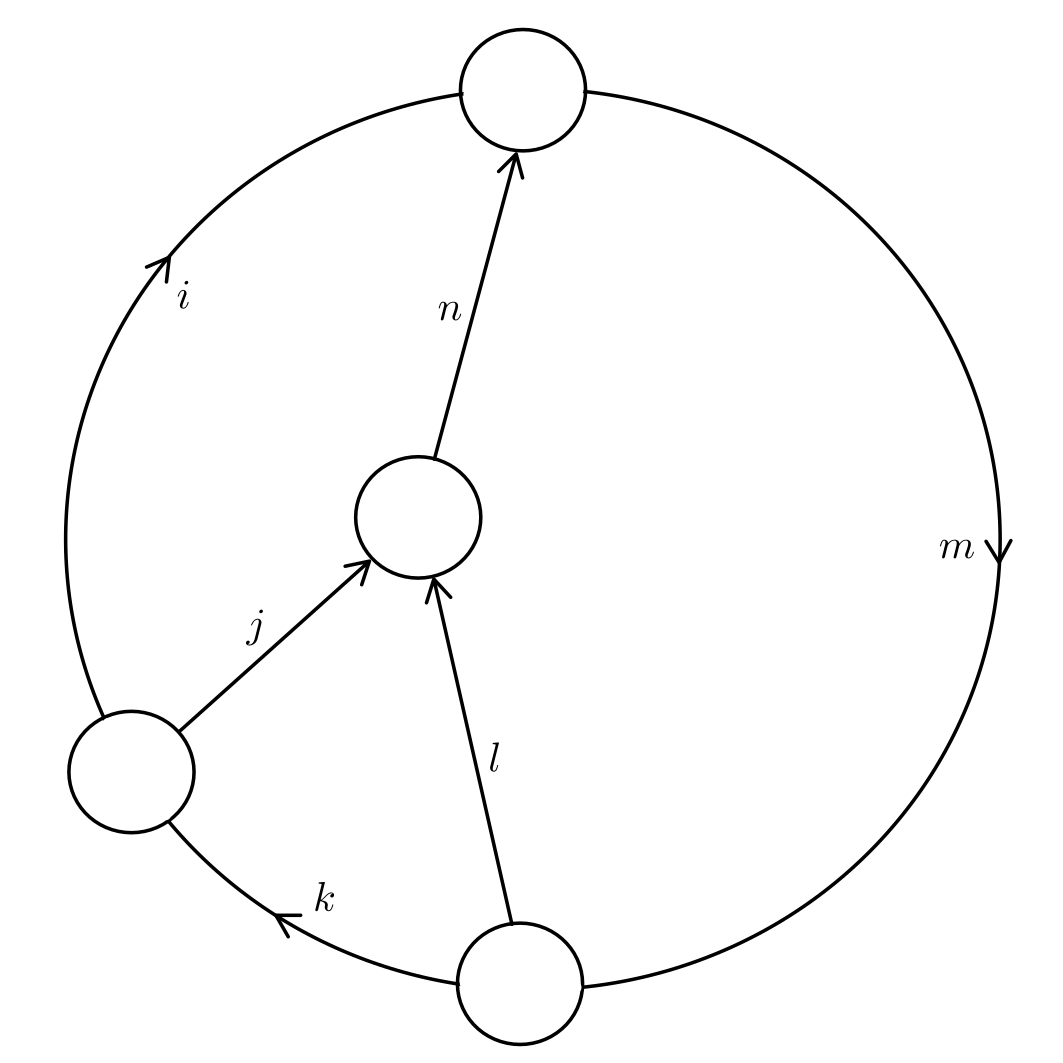
\includegraphics[height=6cm]{6j-geometric}
  \end{center}

  \noindent Using the canonical identifications, we define the
  induced map
  $$\normalizedSixJSymbol{i}{j}{k}{l}{m}{n}: H(i,j,k^{\star}) \otimes H(k,l,m^{\star}) \otimes H(n,l^{\star},j^{\star}) \otimes H(m,n^{\star},i^{\star}) \to \mathbb{k}$$
  to be the normalized $6$j-symbol.
\end{definition}

\begin{proposition}[basic equalities of $6$j symbols]\label{prop/basic-equalities-of-6j-symbols}
  Let $C$ be a (coordinated) premodular category, $I$ its set of
  simples, $i, j, k, k', l, m \in I$,
  $j_{0}, j_{1}, \ldots, j_{8} \in I$, and $\delta$ be the Kronecker
  delta. Then we have the degenerated $6$j symbol
  \begin{equation}\label{eqn/degenerated-6j}
    \normalizedSixJSymbol{i}{j}{k}{l}{m}{0} = \delta_{m,i} \delta_{l,j^{\star}}dim'(i)^{-1}dim'(j)^{-1}Id(i,j,k^{\star})
    \in H(i,j,k^{\star}) \otimes_{\mathbb{k}} H(i^{\star}, j^{\star}, k)
    .
  \end{equation}
  We also have the so called Biedenharn-Elliott identity as an
  equality in the non-ordered tensor product of the
  $\mathbb{k}$-modules
  $$
  H(j_{3}^{\star}, j_{5}^{\star}, j_{6}) \otimes
  H(j_{1}^{\star}, j_{2}^{\star}, j_{5}) \otimes
  H(j_{4}^{\star}, j_{6}^{\star}, j_{0}) \otimes
  H(j_{0}^{\star}, j_{1}, j_{7}) \otimes
  H(j_{7}^{\star}, j_{2}, j_{8}) \otimes
  H(j_{8}^{\star}, j_{3}, j_{4})
  $$
  (in the context of state sum over a triangulation, this
  corresponds to the Pachner $(2,3)$-move):
  \begin{equation}\label{eqn/Biedenharn-Elliot-identity}
    \ast_{j_{0}^{\star}j_{5}j_{8}}
    \left(
      \normalizedSixJSymbol{j_{5}}{j_{3}}{j_{6}}{j_{4}}{j_{0}}{j_{8}} \otimes \normalizedSixJSymbol{j_{1}}{j_{2}}{j_{5}}{j_{8}}{j_{0}}{j_{7}}
    \right)
    =
    \sum_{j \in I} dim(j)
    \ast_{j^{\star}j_{2}j_{3}}\ast_{jj_{4}j_{7}^{\star}}\ast_{jj_{1}j_{6}^{\star}}
    \left(
      \normalizedSixJSymbol{j_{1}}{j_{2}}{j_{5}}{j_{3}}{j_{6}}{j} \otimes
      \normalizedSixJSymbol{j_{1}}{j}{j_{6}}{j_{4}}{j_{0}}{j_{7}} \otimes
      \normalizedSixJSymbol{j_{2}}{j_{3}}{j}{j_{4}}{j_{7}}{j_{8}}
    \right).
  \end{equation}
  We also have the orthonormality relation
  \begin{equation}\label{eqn/orthonormality-relation}
    \delta_{k,k'} Id(i,j,k^{\star}) \otimes Id(k,l,m^{\star})
    =
    dim(k)\,\sum_{n \in I} dim(n) \ast_{im^{\star}n} \ast_{jln^{\star}}
    \left(
      \normalizedSixJSymbol{i^{\star}}{j^{\star}}{k^{\star}}{l^{\star}}{m^{\star}}{n^{\star}} \otimes
      \normalizedSixJSymbol{i}{j}{k'}{l}{m}{n}
    \right).
  \end{equation}
  Finally, we have the Racah identity
  \begin{equation}\label{eqn/Racah-identity}
    \nu'_{j_{3}} \nu'_{j_{6}} (\nu'_{j_{1}} \nu'_{j_{2}} \nu'_{j_{4}} \nu'_{j_{5}})^{-1}
    \normalizedSixJSymbol{j_{1}}{j_{2}}{j_{3}}{j_{4}}{j_{5}}{j_{6}}
    =
    \sum_{j \in I} (\nu'_{j})^{-1} dim(j) \ast_{j^{\star}j_{1}j_{4}} \ast_{jj_{2}j_{5}^{\star}}
    \left(
      \normalizedSixJSymbol{j_{1}}{j_{4}}{j}{j_{2}}{j_{5}}{j_{6}} \otimes
      \normalizedSixJSymbol{j_{2}}{j_{1}}{j_{3}}{j_{4}}{j_{5}}{j}
    \right)
  \end{equation}
\end{proposition}

\begin{proof}
  Proofs and references for the modular case can be found in
  \cite[section VI.5.4]{turaev-qiok-3-manifolds}. The proof does
  not use modularity at all, so it carries through for the
  premodular case verbatim.
\end{proof}

\begin{definition}[$10$j-symbol]\label{def/10j-symbol}
  Let $C$ be a (coordinated) premodular category, $I$ its set of
  simples, and $j_{ab} \in I$ with $j_{ab} = j_{ba}^{\star}$ for
  $0 \leq a, b \leq 4$.
  Wenote $[x,y,z,w]$ to be
  $Hom_{Z}(V_{0}, V_{j_{x}} \otimes V_{j_{y}} \otimes V_{j_{z}} \otimes V_{j_{w}})$.
  Then define the (algebraic) $10$j symbol
  $$
  \tenJSymbol{j_{01}}{j_{02}}{j_{03}}{j_{04}}{j_{12}}{j_{13}}{j_{14}}{{j_{23}}{j_{24}}{j_{34}}}
  $$
  to be the $\mathbb{k}$-linear map from the non-ordered tensor
  product of $\mathbb{k}$-modules
  $$
  [01,02,03,04] \otimes
  [12,13,14,10] \otimes
  [23,24,20,21] \otimes
  [34,30,31,32] \otimes
  [40,41,42,43]
  $$
  % \begin{itemize}
  %   \item
  %         $Hom_{C}(V_{0}, V_{01} \otimes V_{02} \otimes V_{03} \otimes V_{04})$
  %   \item
  %         $Hom_{C}(V_{0}, V_{12} \otimes V_{13} \otimes V_{14} \otimes V_{01}^{\star})$
  %   \item
  %         $Hom_{C}(V_{0}, V_{23} \otimes V_{24} \otimes V_{02}^{\star} \otimes V_{12}^{\star})$
  %   \item
  %         $Hom_{C}(V_{0}, V_{34} \otimes V_{03}^{\star} \otimes V_{13}^{\star} \otimes V_{23}^{\star})$
  %   \item
  %         $Hom_{C}(V_{0}, V_{04}^{\star} \otimes V_{14}^{\star} \otimes V_{24}^{\star} \otimes V_{34}^{\star})$
  % \end{itemize}
  to $\mathbb{k}$ induced by the following (equivalent)
  $C$-colored graphs:
  \begin{center}
    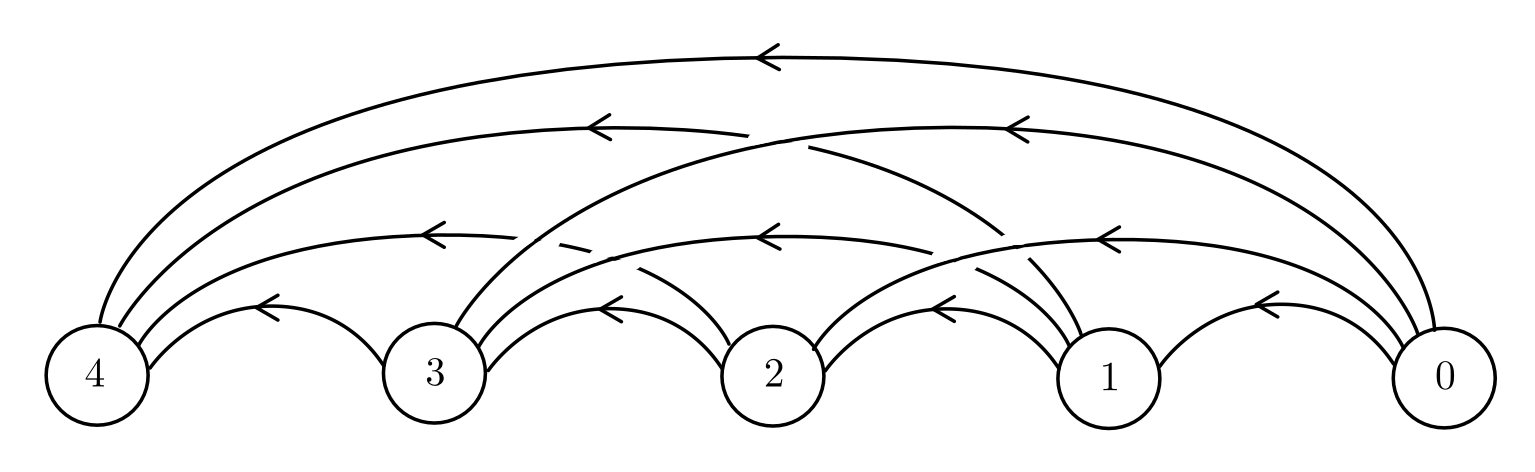
\includegraphics[height=4cm]{10j-plain}
    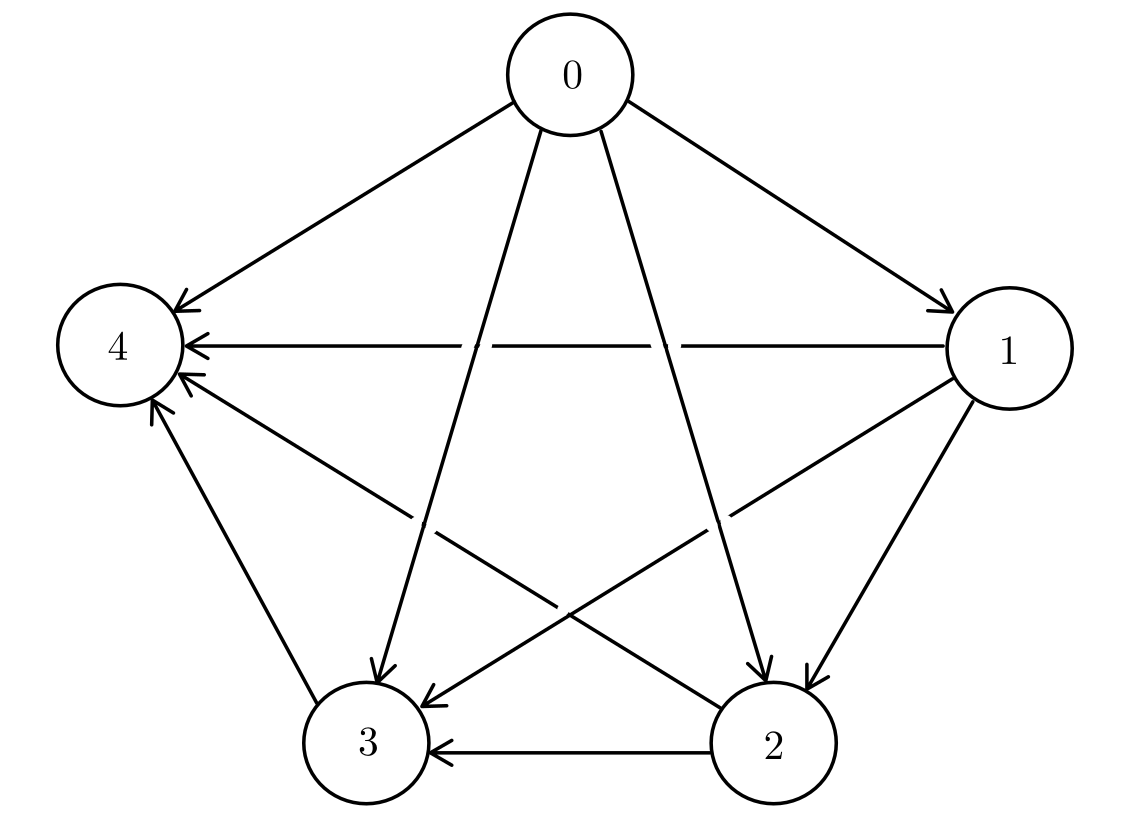
\includegraphics[height=6cm]{10j-geometric}
  \end{center}
\end{definition}

\begin{remark}[$15$j-symbol]\label{remark/15j-symbol}
  A $15$j-symbol is an equivalent variant of a $10$j-symbol used
  in the literature. The $10$j-symbols are more natural, so we
  will not mention nor use the $15$j-symbols in this paper.
\end{remark}

\section{Topology $(T)$}\label{section/topology}
\subsection{$4$-manifold}

Manifolds in real dimension four are of interest because of their
wildness, witnessed in the examples:

\begin{enumerate}
  \item Real dimension $4$ is the first dimension where the
        topological structures, the piecewise-linear structures,
        and the smooth structures disagree.
  \item The euclidean space $\mathbb{R}^{n}$ has exactly one
        smooth structure (up to diffeomorphism) for each
        non-negative integer $n$ except for $\mathbb{R}^{4}$,
        which has more than a countably infinite worth of
        inequivalent smooth structures
        \cite{scorpan/the-wild-world-of-4-manifolds}.
  \item The Poincare conjecture for the $n$-dimensional sphere
        $S^{n}$ has been resolved except for $n=4$, which remains
        widely open to date.
  \item The Universe where we live seems to be best-modeled by a
        $4$-manifold.
\end{enumerate}

\noindent Despite the wildness, Kirby and Siebenmann [TODO: cite
carefully \cite{kirby-siebenmann}] show that the category of
smooth manifolds is equivalent to the category of
piecewise-linear manifolds. The data of the later are smaller and
more elegant. Thus we will really be working on the
piecewise-linear case. By a manifold we mean a piecewise-linear,
oriented, connected and closed manifold in real dimension $4$
unless further specified.

\subsection{Triangulation} \label{subsection/triangulation}

\noindent The standard oriented $4$-simplex is defined to be the
following topological subspace
$$\Delta_{4} = \left\{ \, x \in [0,1]^{5} \,\, \middle| \,\, \sum_{i=0}^{4} x_{i} = 1 \, \right\}.$$

Fix an orientation and denote the
oriented $4$-cell by $\Delta_{4}(01234)$. This
induces orientations for its boundary $3$-cells:
$$\Delta_{3}(\widehat{0}) = \Delta_{3}(1234), \Delta_{3}(\widehat{1}) = \Delta_{3}(-0234), \Delta_{3}(\widehat{2}) = \Delta_{3}(0134), \Delta_{3}(\widehat{3}) =  \Delta_{3}(-0124), \Delta_{3}(\widehat{4}) = \Delta_{3}(0123),$$
where $\Delta_{3}(1234)$ denotes the oriented $3$-cell that
misses the vertex on the $0$th axis and so on. For flexibility,
we also denote for example
$$\Delta_{3}(1234) = \Delta_{3}(-2134) = \Delta_{3}(2314) = \Delta_{3}(-3214) \ldots$$

Notice that the boundary $2$-cells do not receive natural
orientations from the oriented $4$-cell. Take the $2$-cell away
from the $3$rd and the $4$th axes for instance. While the
orientation induced from $\Delta_{3}(0123)$ gives
$\Delta_{2}(012)$, that from $\Delta_{3}(-0124)$ gives
$\Delta_{2}(-012)$. Define $\Delta_{2}(\widehat{ij})$ to be the
boundary $2$-cell with orientation induced from
$\Delta_{3}(\widehat{i})$. It is easy to check that
$\Delta_{2}(\widehat{ji}) = -\Delta_{2}(\widehat{ij})$ and if $i<j$
$$\Delta_{2}(\widehat{ij}) = (-1)^{1+i+j}\Delta_{2}(0 \ldots \widehat{i} \ldots \widehat{j} \ldots 4).$$

By a triangulated ($4$-)space we mean a finite collection of
copies of $\Delta$ with a finite collection of identifications of
the pairs of distinct faces. A triangulated $4$-space $S$
naturally gives rise to a piecewise-linear oriented manifold
$|S|$ (up to a PL-homeomorphism).

\begin{definition}[(oriented) triangulation of an oriented
  $4$-manifold]\label{def/triangulation-of-an-oriented-4-manifold}
  Let $X$ be an oriented $4$-manifold. By an oriented
  triangulation of $X$ we mean a triangulated $4$-space $S$ such
  that $|S|$ is PL-homeomorphic to $X$.
\end{definition}

\subsection{Handle decomposition}

\noindent By Morse's theory of extremal points, any smooth
manifold admits a handle decomposition. By Cerf theory, two
handle decompositions present the same manifold (up to
diffeomorphism) if and only if both decomposition data are
related by a finite sequence of handle creations, handle
annihilations, and handle slides
\cite{gompf-stipsicz/4-manifolds-and-kirby-calculus}. A
triangulation of a manifold admits a natural handle decomposition
by taking dual. The correct state sum based on this datum is the
universal state sum \cite{walker/universal-state-sum}; it
transforms a handle decomposition into a number. A useful fact to
notice is that closed $4$-manifolds are reconstructible from
their handles of indices $0$, $1$, and $2$
(\ref{remark/reconstruction-of-4-manifolds}).

\subsection{Shadow}

% TODO (less urgent) - Figure out why we need integer-shadows.

\noindent A shadow is another type of structure that encodes
closed $4$-manifolds. Roughly speaking, a shadow is a
$2$-polyhedron with extra decorations (called gleams) that
remember the twisting data. A $2$-polyhedron is a topological and
combinatorial object that encodes $3$-dimensional manifolds
\cite{matveev/algorithmic-topology-and-classification-of-3-manifolds}.
It is called a pre-foam in the modern literature
\cite{khovanov-robert/foam}.

\begin{definition}[tripod]\label{def/tripod}
  Define the standard tripod to be the topological subspace of
  $\mathbb{R}^{3}$ consisting of the points $(x,y,z)$ such that
  at least two of the entries are zero, and the last entry
  belongs to $[0,1)$. Define a tripod to be any topological space
  homeomorphic to the standard tripod.
\end{definition}

\begin{definition}[cone]\label{def/cone}
  For each topological space $X$, define its standard open cone
  $cone(X)$ to be the quotient space
  $(X \times \mathbb{R_{\geq 0}})/((x,0) \sim (x',0)).$ Define an
  open cone of $X$ to be any topological space homeomorphic to
  $cone(X)$.
\end{definition}

\begin{definition}[local shape]\label{def/local-shape}
  Let $X$ be a topological space and $x \in X$. Denote by $T$ the
  standard tripod and $S$ the $1$-skeleton of the boundary of the
  standard tetrahedron (a trivalent graph with $4$ vertices and
  $6$ edges). Respectively, we say that $x$ is a smooth point, a
  line point, a tetrahedral point, a boundary smooth point, or a
  boundary line point of $X$ if it has a relative neighborhood
  homeomorphic to $(\mathbb{R}^{2},0)$,
  $(T \times \mathbb{R}, (0, 0))$, $(cone(S), (*, 0))$,
  $(\mathbb{R} \times \mathbb{R}_{\geq 0}, (0, 0))$, or
  $(T \times \mathbb{R}_{\geq 0}, (0, 0))$.
\end{definition}

\begin{definition}[simple $2$-polyhedron]\label{def/simple-2-polyhedron}
  A simple $2$-polyhedron with boundary is defined to be a
  piecewise-linear compact CW-complex $P$ of real dimension two,
  such that each of its point $p$ is either a smooth point, a
  line point, a tetrahedral point, a boundary smooth point, or a
  boundary line point. If only the first three types are
  involved, we call $P$ a simple $2$-polyhedron without boundary.
\end{definition}

\begin{definition}[components of a simple $2$-polyhedron]\label{def/components-of-a-simple-2-polyhedron}
  Let $P$ be a simple $2$-polyhedron with boundary. Define the
  set of smooth points (or called interior points) of $P$ to be
  $Int(P)$. Define the set of line points, tetrahedral points,
  and boundary line points to be $sing(P)$. Define the set of
  boundary line points and boundary smooth points to be
  $\partial P$. Call a connected component of $Int(P)$ to be a
  region of $P$; define the set of regions to be $Region(P)$. $P$
  is said to be orientable if each region of $P$ is orientable.
  An orientation of $P$ is an assignment of orientations to each
  of the region.
\end{definition}

\begin{definition}[shadowed $2$-polyhedron]\label{def/shadowed-2-polyhedron}
  Let $P$ be a simple $2$-polyhedron, and $A$ an abelian group
  with a distinguished element $\omega \in A$. We define a shadow
  to be a pair of an orientable $2$-polyhedron $P$ and a map
  (called gleam) $gl: Region(P) \to A$. Unless specified further,
  we assume that $A = \mathbb{Z}\left[\frac{1}{2}\right]$ and
  $\omega = \frac{1}{2}$. We denote $-P$ to be the same simple
  $2$-polyhedron but with all gleams flipped by $(a \mapsto -a)$.
\end{definition}

\noindent For each connected oriented closed surface $\Sigma$ and
each $a \in A$, there is a shadowed $2$-polyhedron $\Sigma_{a}$
which consists of $\Sigma$ with the gleam $a$ assigned to the
only region. For example, $S^{2}_{0}$ denotes the $0$-gleamed
$2$-sphere.

\begin{definition}[nullity of a shadowed $2$-polyhedron]\label{def/nullity-of-a-shadowed-2-polyhedron}\cite[section VIII.5.1]{turaev-qiok-3-manifolds}
  Let $P$ be an oriented shadowed $2$-polyhedron. For each region
  $Y$ of $P$, the contraction map
  $(P / \partial P) \to P / (P \setminus Y)$ and the orientation
  of $Y$ induces a map
  $$H_{2}(P;\partial P) \to \mathbb{Z}; h \mapsto \langle h | Y \rangle.$$
  Define the symmetric bilinear form $\tilde{Q}_{P}$ on
  $H_{2}(P; \partial P)$ by
  $$\tilde{Q}_{P}(h_{1}, h_{2}) = \sum_{Y} \langle h_{1}|Y\rangle \langle h_{2}|Y\rangle gl(Y) \in A$$
  and restrict it to $Q_{P}$ along the natural map
  $H_{2}(P) \to H_{2}(P; \partial P)$ (which is injective by a
  usual argument using long exact sequence). $H_{2}(P)$ is a free
  abelian group, and so is $Ann(Q_{P})$. Finally, define the
  nullity of $P$ to be $null(P) = rank(Ann(Q_{P}))$.
\end{definition}

\noindent We remark that if the shadowed polyhedron comes from a
$4$-manifold $X$, then the bilinear form defined in the previous
definition coincide with the intersection form of $X$
\cite[section IX.5]{turaev-qiok-3-manifolds}.

\begin{definition}[shadow moves]\label{def/shadow-moves}
  \details{\cite[section VIII.1.3, p.369]{turaev-qiok-3-manifolds}}

  TODO: include graphics

  Basic moves P1P2P3

  A general is a finite composition of $P_1^{\pm 1}$..
\end{definition}

\begin{definition}[shadow]\label{def/shadow}
  A shadow is an equivalence class of shadowed $2$-polyhedron $P$
  up to a shadow move. We denote the shadow by $[P]$, and say
  that $P$ represents the shadow $[P]$. (p.370)
\end{definition}

\noindent For two connected shadow $[P]$ and $[P']$, we construct
the shadow $[P]+[P']$ as follows. Arbitrarily identify two
arbitrarily chosen closed disks $D \subset Int(P)$ and
$D' \subset Int(P')$ in $P \coprod P'$, and equip the interior of
$D$ (a new region) with gleam $0$. So defines a simple
$2$-polyhedron and we say that it represents $[P]+[P']$. It is
well-defined by \cite[lemma VIII.2.1.1]{turaev-qiok-3-manifolds}.
For an integer $m \in \mathbb{Z_{\geq 0}}$, we define $m[P]$ as
the sum of $m$-many $[P]$.

\begin{definition}[stable shadow]\label{def/stable-shadow}
  Two connected shadowed polyhedra $P$, $P'$ are called stably
  shadow equivalent if there exists
  $n, n' \in \mathbb{Z_{\geq 0}}$ such that
  $[P] + m[S^{2}_{0}] = [P'] + m'[S^{2}_{0}]$. Extend the
  definition to non-connected ones in an obvious fashion. A
  stable shadow is defined to be a shadowed polyhedron up to
  stable shadow equivalence. Denote the stable shadow of $[P]$ to
  be $stab([P])$.
\end{definition}

\noindent We are ready to present a closed $4$-manifold in terms
of shadows.

\begin{definition}[locally flat $2$-polyhedron in a
  $4$-manifold]\label{def/locally-flat-2-polyhedron-in-a-4-manifold}
  Let $X$ be a closed $4$-manifold. A $2$-polyhedron $P$ in $X$
  is flat at a point $p \in P$ if there exists a neighborhood $U$
  of $p$ in $X$ such that $U \cap P$ lies in a $3$-dimensional
  submanifold of $X$. We say that $P$ is locally flat if it is
  flat at all $p \in P$. (p.394)
\end{definition}

\begin{definition}[skeleton of a $4$-manifold]\label{def/skeleton-of-a-4-manifold}
  Let $X$ be a closed $4$-manifold. A skeleton (p.395) of $X$ is
  a locally flat orientable simple $2$-polyhedron without
  boundary $P$ such that a closed regular neighborhood of it with
  some $3$- and $4$-handles form $X$.
\end{definition}

\noindent For example, the $\mathbb{C}P^{1}$ (standardly
embedded) is a skeleton of $\mathbb{C}P^{2}$. By \cite[theorem
IX.1.5]{turaev-qiok-3-manifolds}, every $4$-manifold has a
skeleton (by compressing the $(0,1,2)$-handles in an arbitrary
handle decomposition).

\begin{definition}[stable shadow of a $4$-manifold]\label{def/stable-shadow-of-a-4-manifold}
  Let $X$ be a closed $4$-manifold. Take a skeleton $P$ of $X$
  and construct a shadowed simple $2$-polyhedron by assigning
  gleams to the regions $\Sigma$ in the following way.
  \begin{enumerate}
    \item If $\Sigma$ is homeomorphic to a closed surface, define
          the gleam to be the self-intersection (which is
          independent of the orientation of $\Sigma$)
          $$([\Sigma] \cdot [\Sigma]) \in H_{0}(X;\mathbb{Z}) = \mathbb{Z} \subset \mathbb{Z}\left[1/2\right].$$
    \item Otherwise, $\Sigma$ is non-compact. Deformation retract
          it to a compact subsurface $\Sigma_{0}$. Denote $N$ to
          be the normal bundle of $\Sigma_{0}$ in $X$. Consider
          the line bundle $l$ over $\partial \Sigma_{0}$ by
          \cite[section VIII.6.2,
          p.397]{turaev-qiok-3-manifolds}, which may be regarded
          as a subbundle of $N|_{\partial \Sigma_{0}}$. The
          circle bundle $\mathbb{P}(N)$ is trivial over
          $\Sigma_{0}$ since the later is of $1$-homotopy type.
          With a choice of an orientation of $\Sigma_{0}$ and
          $X$, $l$ induces a section of
          $\mathbb{P}(N)|_{\partial}$. The obstruction class of
          this section to the whole $\mathbb{P}(N)$ is an element
          of
          $H^{2}(\Sigma_{0}, \partial \Sigma_{0}; \pi_{1}(S^{1})) = \mathbb{Z}$.
          % [TODO (less urgent): Understand this part really.]
          Finally, define the gleam to be the half of the
          resulting integer (which is independent to the choice
          of $\Sigma_{0}$).
  \end{enumerate}
  It is the main theorem of \cite[section
  IX.1.7]{turaev-qiok-3-manifolds} that all shadowed polyhedra
  chosen in such fashion above are all stably shadow equivalent.
  Therefore, it defines the stable shadow $sh(X)$ of the closed
  $4$-manifold $X$.
\end{definition}

\begin{example}
  $sh(\pm\mathbb{C}P^{2}) = stab([S^{2}_{\pm 1}])$ and
  $sh(S^{4}) = stab([S^{2}_{0}])$.
\end{example}

\noindent Recall from \cite[section
IX.4]{turaev-qiok-3-manifolds} that a handle decomposition of a
closed $4$-manifold $X$ gives rise to a shadow of $X$. The
explicit construction will be recalled below in
\ref{def/shadow-of-a-4-manifold-from-a-handle-decomposition},
which will be used to prove our main theorem.

\begin{definition}[skeleton of a $3$-manifold]\label{def/skeleton-of-a-3-manifold}
  Let $Y$ be a closed $3$-manifold. A skeleton of $Y$ is an
  orientable simple $2$-polyhedron without boundary $P \subset Y$
  such that $Y \setminus P$ is a disjoint union of open
  $3$-balls. (p.400)
\end{definition}

\begin{definition}[shadow cone of a framed link in a
  $3$-manifold]\label{def/shadow-cone-of-a-framed-link-in-a-3-manifold}
  \noindent Every compact $3$-manifold $Y$ has a skeleton
  \cite[theorem IX 2.1.1]{turaev-qiok-3-manifolds}. For example,
  the equator $S^{2}$ of $S^{3}$ is a skeleton. Let $P$ be a
  skeleton of $Y$ and $l$ be a framed link in $Y$. Projecting $l$
  generically onto $P$ induces a shadow projection. Assign gleams
  around each crossing point as in \cite[figure
  IX.3.4]{turaev-qiok-3-manifolds}. Then construct the shadow by
  naturally attaching a disk along each projected component on
  $P$ (as a new region) endowed with zero gleam. Denote the
  resulting shadow to be $CO(Y,l)$ (well-defined up to stable
  shadow moves \cite[section IX.3.3]{turaev-qiok-3-manifolds}).
\end{definition}

\begin{definition}[shadow of a $4$-manifold from a handle
  decomposition]\label{def/shadow-of-a-4-manifold-from-a-handle-decomposition}
  Let $X$ be an oriented $4$-manifold and
  $H = \bigcup_{i=0}^{4} H_{i}$ be a handle decomposition, where
  $H_{i}$ denotes the union of the handles of index $i$. Define
  $Y$ to be the closed $3$-manifold $\partial(H_{0} \cup H_{1})$.
  By the definition of handle decomposition, the gluing datum of
  $H_{2}$ onto the handles with lower indices is encoded as a
  link $l$ in $Y$. Define the stable shadow $sh'(X,H)$ to be
  $CO(Y,l)$.
\end{definition}

\begin{remark}\label{remark/stable-shadow-of-a-4-manifold}
  It is a theorem of \cite[IX.4.2]{turaev-qiok-3-manifolds} that
  $sh'(X,H)$ does not depend on the choice of $H$ as a stable
  shadow. In fact, $sh'(X,H)$ equals the stable shadow $sh(X)$
  \cite[IX.7]{turaev-qiok-3-manifolds}.
\end{remark}

\begin{remark}\label{remark/reconstruction-of-4-manifolds}\cite[section 4.4]{gompf-stipsicz/4-manifolds-and-kirby-calculus}
  The handles of indices $\leq 2$ are enough to reconstruct the
  whole closed $4$-manifold.
\end{remark}

\section{Sum $\left( \int_{T}{A} \right)$}\label{section/sum}
\subsection{Crane-Yetter state sum}

\begin{definition}[$C$-colored ($4$-)simplex]\label{def/C-colored-simplex}
  Let $C$ be a (coordinated) premodular category, $I$ be the set
  of simples in $C$, and $\Delta$ be the standard oriented
  $4$-cell $\Delta_{4}(01234)$ defined in section
  \ref{subsection/triangulation}. Define a $C$-coloring on
  $\Delta$ to be a map from the set of oriented $2$-cells of
  $\Delta$ to $I$.
  $\beta(-\Delta_{2}) = \beta(\Delta_{2})^{\star}$. A $C$-colored
  $4$-simplex is a $4$-simplex with a $C$-coloring.
\end{definition}

\begin{definition}[$C$-colored triangulation]\label{def/C-colored-triangulation}
  Let $C$ be a (coordinated) premodular category, $I$ be the set
  of simples in $C$, $X$ be a closed oriented $4$-manifold, and
  $T$ be an (oriented) triangulation of $X$. A $C$-coloring of
  $T$ is an assignment for each $4$-simplex of $T$ a
  $C$-coloring. Define a $C$-colored triangulation to be a
  triangulation with a $C$-coloring.
\end{definition}

\begin{definition}[$10$j symbol for a $C$-colored simplex]\label{def/10j-symbol-for-a-C-colored-simplex}
  Let $\Delta = (\Delta_{4}(01234), \beta)$ be a $C$-colored
  simplex. Denote $\beta_{\widehat{ab}}$ to be the color
  $\beta(\Delta_{2}(\widehat{ab})) \in I$ assigned to the
  oriented $2$-cell $\Delta_{2}(\widehat{ab})$. We define the
  $10$j symbol for $\Delta$ to be the (algebraic) $10$j-symbol
  (\ref{def/10j-symbol})
  $$
  10j(\Delta) =
  \tenJSymbol{\beta_{\widehat{01}}}{\beta_{\widehat{02}}}{\beta_{\widehat{03}}}{\beta_{\widehat{04}}} {\beta_{\widehat{12}}}{\beta_{\widehat{13}}}{\beta_{\widehat{14}}} {{\beta_{\widehat{23}}}{\beta_{\widehat{24}}}{\beta_{\widehat{34}}}}.
  $$
\end{definition}

\begin{definition}[Crane-Yetter state sum for a closed
  $4$-manifold]\label{def/crane-yetter-state-sum-for-a-closed-4-manifold}
  Let $C$ be a (coordinated) premodular category and $X$ a closed
  $4$-manifold. We define the Crane-Yetter state sum for $X$ to
  be
  $$
  \int_{X}^{CY} C = \ast \left( \bigotimes_{\Delta \in T} 10j(\Delta) \right) \in \mathbb{k},
  $$
  [TODO: fix constants (no.. need to redefine the whole thing
  following Walker)] where $T$ denotes an oriented triangulation
  of $X$, and $\ast$ denotes the full contraction induced based
  on the fact that each oriented $3$-simplex is paired with
  another with opposite orientation.
\end{definition}

\noindent The state sum is independent to the choice of $T$, and
thus an invariant for closed $4$-manifolds. In fact, it can be
extended to a fully extended topological quantum field theory
(\cite[section 1.5]{bjs2018} \cite{cooke2019excision}
\cite{integrating-quantum-groups-over-surfaces}
\cite{fac-homo--kirillov-tham}). For explicit evaluations of the
Crane-Yetter model on $4$-manifolds, see
\cite{barenz/evaluation-crane-yetter}; for general $2$-manifolds
(category-valued), see \cite{guu/higher-genera-center}.

\subsection{Shadow state sum} \label{subsection/shadow-state-sum}

Throughout this subsection (\ref{subsection/shadow-state-sum}),
we fix an orientable shadowed $2$-polyhedron $P$ (over
$\mathbb{Z}[1/2]$ with boundary), a (coordinated) premodular
category $C$, and its set of simples $I$. Our goal is to define
the shadow state sum $\int_{P}^{sh} C$.

\begin{definition}[module of a trivalent graph]\label{def/module-of-a-trivalent-graph}
Let $\gamma$ be a trivalent graph. By a $C$-coloring of $\gamma$
we mean a map $\lambda$ from the set of oriented edges of
$\gamma$ to the set $I$ of $C$-simples such that
$\lambda(e) = \lambda(-e)^{\star}$. Denote by $color(\gamma; C)$
the set of all $C$-colorings of $\gamma$. For each $C$-coloring
of the trivalent graph $\gamma$, define a $\mathbb{k}$-module
$$H(\lambda) = \bigotimes_{x} H(i_{x}, i_{x}', i_{x}''),$$
where $x$ runs through all vertices of $\gamma$ and the $i_{x}$'s
denote the colors assigned to the nearby edges oriented toward
$x$. Then define a $\mathbb{k}$-module
$$H(\gamma) = \bigoplus_{\lambda \in color(\gamma; C)} H(\lambda)$$
with the convention that $H(G_{0}) = \mathbb{k}$, where $G_{0}$
denotes the empty graph.
\end{definition}

By a $C$-coloring of $P$ we mean a map $\phi$ from the set of
oriented regions of $P$ to $I$ such that
$\phi(\Sigma) = \phi(-\Sigma)^{\star}$. Denote by $color(P; C)$
the set of all $C$-colorings of $P$.

An orientation of a $2$D region induces an orientation on its
edges by $(\vec{n} \wedge -)$, where $\vec{n}$ denotes a vector
pointing outward from the region. Therefore, a $C$-coloring
$\phi$ of $P$ induces a $C$-coloring $\partial \phi$ of its
boundary $\partial P$.

\begin{definition}[shadow state sum]\label{def/shadow-state-sum}\details{\cite[section X.1.2]{turaev-qiok-3-manifolds}}
  Every $C$-coloring on the boundary of a $2$-polyhedron extends
  to some $C$-coloring on it, so
  $H(\partial P) = \sum_{\phi \in color(P; C)} H(\partial \phi)$.
  Fix a $\phi \in color(P; C)$, and define the following
  $\mathbb{k}$-modules and vectors.
\begin{itemize}
  \item For each oriented edge $\vec{e}$ in $P$ that does not lie
        in $\partial P$, define $H_{\phi}(\vec{e})$ to be
        $H(i,i',i'')$ where the $i$'s are the colors assigned to
        the nearby region compatibly oriented with $\vec{e}$.
  \item For each (unoriented) edge $e$ in $P$ that does not lie
        in $\partial P$, define $H_{\phi}(e)$ to be the
        non-ordered tensor product
        $H_{\phi}(\vec{e}) \otimes H_{\phi}(-\vec{e})$ with an
        arbitrary orientation. Use the pairing
        \ref{def/contraction} to define a canonical vector
        $|e|_{\phi} \in H_{\phi}(e)$.
  \item For each tetrahedral point $x \in P$, pick a small enough
        neighborhood of $x$ in $P$ homeomorphic to the cone of
        the $1$-skeleton of the boundary of some tetrahedron.
        Clearly, this is also a $C$-colored $2$-polyhedron with
        four boundary line points $x_{0}, x_{1}, x_{2}, x_{3}$
        and six $C$-colored regions. Denote by $\phi_{ij}$ the
        color for the oriented region
        $\overrightarrow{xx_{i}x_{j}}$; clearly,
        $\phi_{ij} = \phi_{ji}^{\star}$. Finally, define the pair
        of vector and $\mathbb{k}$-module for $x$ to
        be $$|x|_{\phi} := \normalizedSixJSymbol{\phi_{01}}{\phi_{02}}{\phi_{30}}{\phi_{32}}{\phi_{13}}{\phi_{21}} \in \bigotimes_{i=0}^{3} H_{\phi}(\overrightarrow{x_{i}x}) =: H_{\phi}(x),$$
        where $\otimes$ denotes the unordered tensor product of
        $\mathbb{k}$-modules. (Notice that the result is
        independent to the labeling $0, 1, 2, 3$.)
\end{itemize}

\noindent The procedure above defines a vector in the
$\mathbb{k}$-module
$$\left( \bigotimes_{x} H_{\phi}(x) \right) \otimes \left( \bigotimes_{e} H_{\phi}(e) \right)$$
where $x$ runs over the tetrahedral points of $P$ and $e$ runs
over the (nonoriented) edges of $P$ that does not lie entirely in
$\partial P$. By contracting the vector along each edge $e$ whose
boundary points are not both in $\partial P$, we obtain a vector
in $|\phi| \in H(\partial \phi)$. Finally, we define the shadow state sum
to be
$$\int^{sh}_{P} C = D^{-b_{2}(P) - null(P)} \sum_{\phi \in color(P)} \sigma_{\phi} |\phi| \in \sum_{\phi} H(\partial \phi) = H(\partial P),$$
where $b_{2}$ denotes the second betti number, $null$ denotes the
nullity (\ref{def/nullity-of-a-shadowed-2-polyhedron}), and
$\sigma_{\phi} \in \mathbb{k}$ is a normalizing constant defined
assign as
$$\sigma_{\phi} = \prod_{e} dim_{C}'(\partial\phi(e))^{-1} \prod_{Y} dim_{C}(\phi(Y))^{\chi(Y)} \nu'_{\phi}(Y)^{2gl(Y)} \prod_{g} dim_{\mathbb{k}}(Hom_{C}(V_{0}, V_{i} \otimes V_{j} \otimes V_{k})),$$
where $e$ runs over edges of $\partial P$ (but not circle
$1$-strata), $Y$ runs over regions of $X$, $g$ runs over circle
$1$-strata of $sing(X)$, and $\chi$ denotes the Euler
characteristics.
\end{definition}

\begin{proposition}[shadow state sum is invariant under stable
  shadow
  move]\label{prop/shadow-state-sum-is-invariant-under-stable-shadow-move}
  Let $C$ be a premodular category and $P, P'$ be $2$-polyhedra
  that are equal as stable shadows. Then
  $$\int^{sh}_{P} C = \int^{sh}_{P'} C.$$
  Namely, shadow state sum is invariant under stable shadow move.
\end{proposition}
\begin{proof}
  We start with the special case where $C$ is a modular category.
  For invariance under basic shadow moves, the essential
  ingredients are the orthonormality relation, the Racah
  identity, and the Biedenharn-Elliott identity
  (\ref{prop/basic-equalities-of-6j-symbols}). See \cite[theorem
  X.2.1]{turaev-qiok-3-manifolds} for a proof. For invariance
  under addition of $S^{2}_{0}$, it boils down to proving the
  addition formula $$|P_{1} + P_{2}| = |P_{1}| \otimes |P_{2}|$$
  \cite[theorem X.2.2]{turaev-qiok-3-manifolds} and using the
  equality $|S^{2}_{0}| = D^{-2} \sum_{i \in I} dim(i)^{2} = 1$.
  Both proofs carry through verbatim to the premodular case.
\end{proof}

% TODO (less urgent): Provide explicit examples. This is
% important for expositing.

\begin{definition}[shadow state sum of a $4$-manifold]\label{def/shadow-state-sum-of-a-4-manifold}
  Let $X$ be a closed $4$-manifold, $C$ a (coordinated)
  premodular category, $stab([P])$ a stable shadow of $X$
  represented by a shadowed $2$-polyhedron $P$. Define the shadow
  state sum $\int_{X}^{sh} C$ of $X$ to be $\int_{P}^{sh} C$. It
  is well-defined by \ref{remark/stable-shadow-of-a-4-manifold}
  and
  \ref{proposition/shadow-state-sum-is-invariant-under-stable-shadow-move}.
\end{definition}

\begin{proposition}[shadow state sum is local]\label{prop/shadow-state-sum-is-local}
  [TODO: need to fix the CY state sum first.. and I need to prove
  this by myself as it doesn't seem to be proven in Turaev's
  book.]
\end{proposition}

\noindent We end the subsection with the key lemma.

\begin{lemma}[$10$j symbol as a shadow state sum]\label{lemma/10j-symbol-as-shadow-state-sum}
  [TODO: include many graphics]
\end{lemma}

\subsection{Main result: equivalence of state sums}

\noindent We state and prove the main theorem of this paper. See
\ref{subsection/a-summary-to-experts} for the main idea of the
proof.

\begin{theorem}[equivalence of state sums]
  Let $X$ be a closed $4$-manifold and $C$ be a (coordinated)
  premodular category. Then
  $$\int^{CY}_{X}C = \int^{sh}_{X} C.$$
  Namely, their Crane-Yetter state sum and shadow state sum are
  equal.
\end{theorem}

\begin{proof}
  Let $\epsilon > 0$ (very small), $T$ be a triangulation of $X$,
  and $H = \bigcup_{i=0}^{4} H_{i}$ be a dual handle
  decomposition in which the attaching region of each $1$-handle
  on each $0$-handle is the $\epsilon$-ball ($3$-dimensional) of
  the central point of corresponding $3$-cell. (This makes sense
  because we have realized the standard $4$-cell as a subspace of
  the standard $\mathbb{R}^{5}$ in
  (\ref{subsection/triangulation}).) To compute the shadow state
  sum, we first need to construct a shadow for $X$. We will
  construct it by the procedure given in
  \ref{def/shadow-of-a-4-manifold-from-a-handle-decomposition} as
  the resulting shadow will resemble the structure of $T$.

  Suppose $T$ has $n$ $4$-cells. Let $\Delta$ be a $4$-cell in
  $T$. It corresponds to a $0$-handle $h_{0}$. Each of the
  $3$-cell $\delta$ among the five in $\partial \Delta$
  corresponds to (a half of) a $1$-handle $h_{1}$, which is glued
  to $h_{0}$. Hence $H_{0} \cup H_{1}$ is a solid $4$-body with
  $n$ $0$-cells and $\frac{5n}{2}$ $1$-cells. The $3$-manifold
  $Y = \partial(H_{0} \cup H_{1})$ in the
  construction \ref{def/shadow-of-a-4-manifold-from-a-handle-decomposition}
  is therefore homeomorphic to the space constructed as follows:
  First take the union of $n$ $3$-spheres identified to the
  $0$-cells, and connected sum any pair of them if and only if
  the corresponding $0$-cells are connected by $1$-cells. It is
  also homeomorphic to a union of $n$ $S^{3} - B^{3} \times 5$
  (denoted by $S_{0,5}$) with obvious parts that overlap, where
  the $B^{3}$ can be identified as the $\epsilon$-ball introduced
  above.

  Following the construction, we will construct a skeleton for
  the $3$-manifold $Y$. The construction will be first carried
  out locally in each $S_{0,5}$, and then glued together with
  some modification:

  \begin{enumerate}
    \item In each $S_{0,5}$, fix a $3$-ball $B$ of size
          $\epsilon$ such that the following condition holds. For
          each removed $B^{3}$, pick a shortest path from its
          center to the center of $B$. Thicken each path to have
          width radius $\frac{\epsilon}{2}$. We require that the
          five thicken paths do not intersect each other. The
          boundary of the union is a $5$-punctured sphere
          $\Sigma_{0,5}$ in $S_{0,5}$.
    \item Identify arbitrarily the end of a $5$-punctured sphere
          (a circle) with the end of another $5$-punctured sphere
          (another circle) if this pair corresponds to the same
          $1$-handle.
    \item For each identified circle, glue a $2$-disk along its
          boundary.
  \end{enumerate}

  The resulting polyhedron $P$ is simple and orientable.
  Moreover, its complement in $Y$ is a union of open $3$-balls.
  Therefore, $P$ is a skeleton for the $3$-manifold $Y$ as
  desired.

  The next step in the construction
  (\ref{def/shadow-of-a-4-manifold-from-a-handle-decomposition}) is
  to project the link $l \subset Y$ as the gluing datum of
  $H_{2}$ onto $\partial(H_{0} \cup H_{1})$. As the handle
  decomposition $H$ comes from a triangulation, the links are
  identical in each local piece $S^{3} - B^{3} \times 5$. A
  simple geometric exercise shows that a generic projection of
  $l$ onto $P$ looks as follows (with gleams added as in the
  construction
  \ref{def/shadow-of-a-4-manifold-from-a-handle-decomposition}).

  \noindent [TODO: Add graphic [20220217T143000 (1)]]

  Using \ref{prop/shadow-state-sum-is-local}, it remains to show
  that the shadow state sum of the (local) shadow depicted above
  coincides with the $10$j symbol. This is exactly what the key
  lemma \ref{lemma/10j-symbol-as-shadow-state-sum} shows, which completes the proof.
\end{proof}
